\section{Säure-Base-Reaktionen $pK_{s}+ pK_{b} = 14$}
Ein \textbf{Ampholyt} ist ein Teilchen das sowohl als Säure, wie auch als Base Wirken kann. 
Z.b. \ce{ H2O, HSO4^-, HS-}
\subsection{Säure-Base GGW}
    \begin{minipage}{0.65\columnwidth}
        Bergab = GGW rechts: \ce{ HCl + H2O <=>> Cl- + H3O+ }

        Bergauf = GGW links: \ce{ HS- + H2O <<=> S^{2-} + H3O+ }
    \end{minipage}
    \hfill
    \begin{minipage}{0.33\columnwidth}
        \textbf{S}äuren = Protonen\textbf{s}pender

        \textbf{B}asen = Protonen\textbf{b}inder
    \end{minipage}

\subsection{pH-Wert}
    \begin{minipage}{0.4\columnwidth}
        \begin{itemize}
            \item Aussage über \textbf{Gehalt} von \ce{H3O+}
            \item liegt zwischen 0 und 14
            \item \ce{[H3O+]} = $10^{-pH}$
        \end{itemize}
    \end{minipage}
    \hfill
    \begin{minipage}{0.59\columnwidth}
        \begin{itemize}
            \item \textbf{keine} Aussage über Säurestärke
            \item gilt für verdünnte, wässrige Lösungen ($\geq$ 1mol/L)
            \item \ce{[OH^-]} = $10^{-14+pH}$
        \end{itemize}
    \end{minipage}
    
    Neutralisation: $\underbrace{\ce{\textcolor{red}{H_3O^+} + {Cl^-}}}_{\text{Salzsäure}} + \underbrace{\ce{{Na^+} + \textcolor{green}{OH^-}}}_{\text{Natronlauge}} \ce{->} \underbrace{\ce{\textcolor{blue}{2 H_2O}}}_{\text{Wasser}} + \underbrace{\ce{{Cl^-} + {Na^+}}}_{\text{Kochsalz-Lsg.}}$

\subsection{Protolyse - Säure, Base Reaktion}
\begin{enumerate}
	\item Welche ist Säure, welche Base? (welches nimmt H, welches gibt H)
	\item Reagiert es? -> Säure und Base reagieren dann miteinander, wenn sie in Bergab-Stellung stehen (GGW rechts), ansonsten ist sie nicht stark.
	\item Reaktionsgleichung aufstellen
	\item H zur konjugierten Säure hinzufügen und von Säure entziehen.
	\item Ladungen überprüfen (negative Ladung = mehr Elektronen als Protonen und positive Ladung = weniger Elektronen als Protonen)
\end{enumerate}

\begin{center}
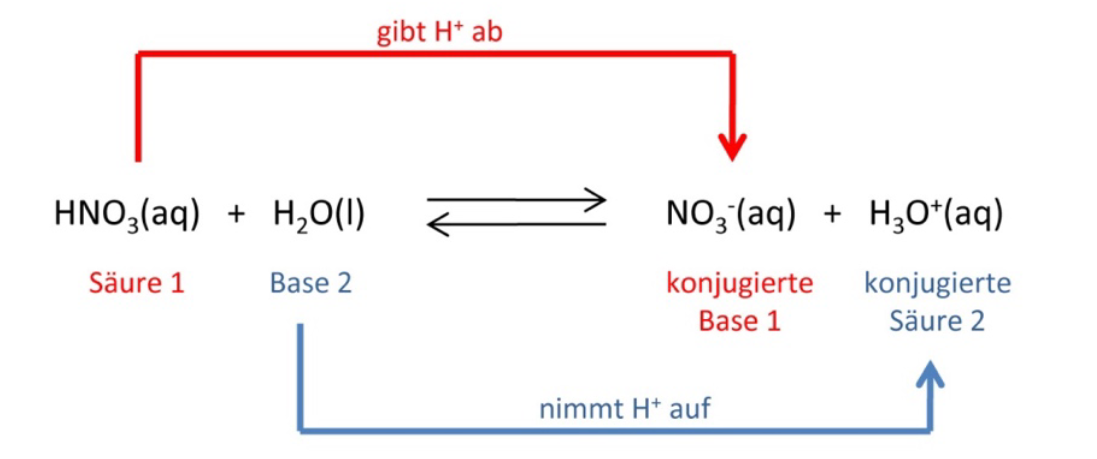
\includegraphics[scale=0.2]{pictures/Saure_Base_ex.png}
\end{center}
